% This is LLNCS.DEM the demonstration file of
% the LaTeX macro package from Springer-Verlag
% for Lecture Notes in Computer Science,
% version 2.4 for LaTeX2e as of 16. April 2010
%
\documentclass{llncs}
%
\usepackage{makeidx}  % allows for indexgeneration
\usepackage{epsfig} % allows encoding PostScript images
%
\begin{document}
%
\frontmatter          % for the preliminaries
%
\pagestyle{headings}  % switches on printing of running heads
\mainmatter              % start of the contributions
%
\title{Fiber feature map based landmark initialization for highly deformable DTI registration}
\author{Aditya Gupta$^{1,3}$, Matthew Toews$^{2}$, Ravikiran Janardhana$^{4}$, Yogesh Rathi$^{2}$, John Gilmore$^{3}$, Maria Escolar$^{1}$, Martin Styner$^{3,4}$}


\institute{$^{1}$ Dept Pediatrics, University of Pittsburgh, PA, USA; ${^2}$ Harvard Medical School, Boston MA; ${^3}$ Dept Psychiatry, ${^4}$ Dept Computer Science, University of North Carolina, Chapel Hill, NC}


\maketitle              % typeset the title of the contribution

% begin abstract

\begin{abstract}
This paper presents a novel pipeline for the registration of diffusion tensor images (DTI) with large pathological
variations to normal controls based on the use of a novel feature map derived from white matter (WM) fiber
tracts. The research presented aims towards an atlas based DTI analysis of subjects with considerable brain
pathologies such as tumors or hydrocephalus. In this paper, we propose a novel feature map that is robust against
variations in WM fiber tract integrity and use these feature maps to determine a landmark correspondence using
a 3D point correspondence algorithm. This correspondence drives a deformation field computed using Gaussian
radial basis functions(RBF). This field is employed as an initialization to a standard deformable registration
method like demons. We present early preliminary results on the registration of a normal control dataset to a
dataset with abnormally enlarged lateral ventricles affected by fatal demyelinating Krabbe disease. The results
are analyzed based on a regional tensor matching criterion and a visual assessment of overlap of major WM fiber
tracts. While further evaluation and improvements are necessary, the results presented in this paper highlight
the potential of our method in handling registration of subjects with severe WM pathology.

\keywords{fiber feature map, 3D point correspondence, DTI, large deformation fields}
\end{abstract}

% end abstract


% begin introduction
% end introduction

\section{Introduction}

\section{Method}
Lorem ipsum dolor sit amet, dolorem forensibus cum no, sed mucius quodsi legimus ei, malorum intellegebat ei pro. 
Ignota forensibus ei per, velit apeirian adipiscing qui no, id everti aliquid has. Scripta delicatissimi per at, 
mea rebum omnes cu. Et vim falli error mundi, oratio ignota quaerendum usu in. 

%
\subsection{Feature Map Generation}
%
In this section, we present the steps involved in generating the feature
map from the raw diffusion weighted image (DWI) and the image mask. First,
we perform a 2-tensor unscented kalman filter based tractography \cite{malc:mic} inorder 
to obtain the fiber tracts image. Once the fiber tracts have been generated, 
we compute two main features namely, number of fiber segments per voxel and 
entropy of fiber orientations per voxel.  We normalize and combine these two features 
inorder to develop the feature image. The following sections describe each step of 
the feature map generation in detail.

%
\subsubsection{Fiber Tracts Generation}
%
The fiber tracts are generated from the raw DWI image and the image mask by performing
a 2-tensor unscented kalman filter (ukf) based tractography. Unlike many of the existing 
techniques, in ukf-based tractography, fiber tracking is formulated as causal estimation; 
at each step of tracing the fiber, the current estimate of the signal is guided by the
previous. To do this, the signal is modeled as a discrete mixture of Watson directional
functions and tractography is performed within a filtering framework. Starting from
a seed point, each fiber is traced to its termination using an unscented Kalman filter 
to simultaneously fit the signal and propagate in the most consistent direction. Despite the 
presence of noise and uncertainty, this provides an accurate estimate of the local structure 
at each point along the fiber. The in-depth details of the tractography can be found in \cite{malc:mic}.
While generating the fiber tracts for our experiments, we configured the number of seeds per 
voxel as 8, seed FA limit as 0.18, minimum FA to continue tractography as 0.12 and branching
was suppressed while using multiple tensors. 

%
\subsubsection{Fiber Segments per voxel}
%
In this step, we traverse through all the fiber segments in the fiber tracts generated and 
identify which voxel a particular fiber segment belongs to and increment its counter by one. 
The result of this step is an image where the value at a particular voxel indicates the number
of fiber segments it contains and thus indicates the density of fibers at that voxel.

%
\subsubsection{Entropy of Fiber Orientations}
%
In order to compute the entropy of fiber orientations at a particular voxel, we first need to define
what is the fiber orientation at a voxel. Consider the below example in Figure 1, where a single fiber 
passes through the fiber points p1, p2 and p3 at a particular voxel. The fiber orientation at a
fiber point is defined as the direction of the tangent joining its neighboring fiber segment points. At
the boundary fiber points, the fiber orientation is defined as the direction of the line connecting it to the previous
or subsequent fiber point. The fiber orientation at a voxel can now be defined as a tuple of fiber orientations at 
the fiber points contained in the voxel.

% Figure 1
\begin{figure}
\centering
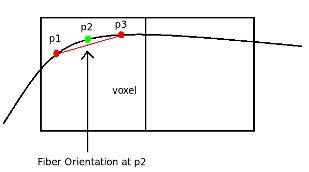
\epsfig{file=images/fiberorientation.png}
\caption{The figure depicts the fiber orientation computed at fiber segment point p2 i.e., the tangential
direction connecting its neighboring fiber segment points p1 and p3.}
\end{figure}
%
The next step is to compute the histogram (see Figure 2) of these fiber orientations at each voxel. This histogram computed
is on a unit sphere which is subdivided into equal regions by fitting a platonic solid such as an icosahedron onto
the surface of the sphere with a sub-division level of 6.  At the subdivision level of 6, we get 492 icosahedron 
vertices and given a fiber orientation, we approximate it to a particular icosahedron triangular face and add it to the 
icosahedron vertices using barycentric coordinate system in which the location of the fiber direction is specified 
as the center of mass, or barycenter, of masses placed at the vertices of a simplex i.e., a triangle in our case.

% Figure 2
\begin{figure}
\centering
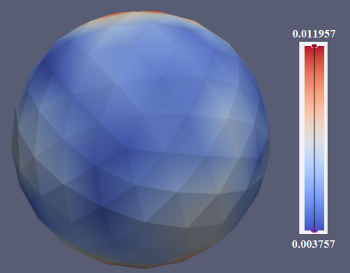
\epsfig{file=images/histo.png}
\caption{The figure shows the histogram representing the fiber orientations of a particular voxel on a unit sphere which
is subdivided into equal regions by fitting a icosahedron onto the surface of the sphere.}
\end{figure}
%
This histogram is then used to generate the entropy of fiber orientations. Entropy is a measure of disorder, or more 
precisely unpredictability.  For example, a series of coin tosses with a fair coin has maximum entropy, since there 
is no way to predict what will come next. A string of coin tosses with a coin with two heads and no tails has zero 
entropy, since the coin will always come up heads. Similarly if there is just a single track fiber, there is less 
unpredictability and hence lower entropy and if there are multiple fiber tracts and multiple fiber orientations, 
this means that there is more unpredictability and hence higher entropy. 
 
Using the histogram, we compute entropy of fiber orientations per voxel as below: 
 
\begin{equation}
H(X) = - \sum_{i=1}^n p(x_i) \log_{b} p(x_i) 
\end{equation}

where, \textit{H(X)} is the entropy of fiber orientation at a particular voxel, \textit{p(x$_{i}$)} is the probability of a fiber 
orientation to be \textit{x$_{i}$} and \textit{n} represents all possible fiber orientations. 

%
\subsubsection{Combining features to obtain Feature Map}
%
In order to obtain the feature map, we first normalize the two features namely fiber segments per voxel and entropy
of fiber orientations per voxel by dividing each of these by their respective maximum. The feature map is then obtained
by computing the square root of the product of normalized values of the two features.

%Equation
\begin{equation}
F_i(X) = \sqrt {\frac{H_i(X)}{max  H(X)} * \frac{fs_i(X)}{max  fs(X)} }
\end{equation}

where \textit{F$_i$(X)}, \textit{H$_i$(X)} and \textit{fs$_i$(X)} are the feature map value, entropy of fiber orientations 
and the number of fiber segments at voxel \textit{i} respectively, \textit{max H(X)} and \textit{max fs(X)} are the maximum values of
entropy of fiber orientations and number of fiber segments over the entire image. 

This feature map is certain to highlight the crossing fiber landmarks which can further be used for DTI registration.
If one examines the fiber segments per voxel image, it is bound to have higher intensities in those regions where there
are large number of single fiber tracts and multiple fiber tracts and lower intensities in regions of fewer or no fiber tracts.
The entropy of fiber orientations image has higher intensities in regions of dispersed single fiber tracts and crossing fiber 
tracts (due to greater variation in fiber orientations) and lower intensities in uni-directional single fiber tracts or no fiber 
tracts regions. Hence, by combining these two, we can negate out the uni-directional single fiber tracts and no fiber tracts regions, 
thus highlighting the crossing fiber regions or landmarks.

\section{Results}
\subsection{Feature Images}
Lorem ipsum dolor sit amet, dolorem forensibus cum no, sed mucius quodsi legimus ei, malorum intellegebat ei pro. 
Ignota forensibus ei per, velit apeirian adipiscing qui no, id everti aliquid has. Scripta delicatissimi per at, 
mLorem ipsum dolor sit amet, dolorem forensibus cum no, sed mucius quodsi legimus ei, malorum intellegebat ei pro. 
Ignota forensibus ei per, velit apeirian adipiscing qui no, id everti aliquid has. Scripta delicatissimi per at, 
mea rebum omnes cu. Et vim falli error mundi, oratio ignota quaerendum usu in. 

% Figure 3
\begin{figure}
\centering
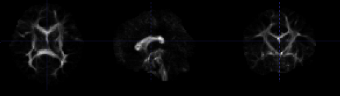
\epsfig{file=images/fs_final.png}
\caption{Fiber Segments per voxel image}
\end{figure}

% Figure 4
\begin{figure}
\centering
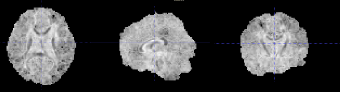
\epsfig{file=images/entropy_final.png}
\caption{Entropy of fiber orientations per voxel image}
\end{figure}

% Figure 5
\begin{figure}
\centering
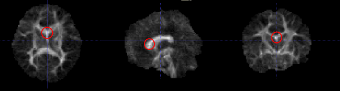
\epsfig{file=images/combined_final_with_landmarks.png}
\caption{This figure shows the combined feature map image. The crossing fiber landmarks which have higher intensities are also highlighted in this image}
\end{figure}

%
% ---- Bibliography ----
%
\begin{thebibliography}{}
%
\bibitem {malc:mic}
James G. Malcolm, Oleg Michailovich, Sylvain Bouix, Carl-Fredrik Westin, Martha E. Shenton, Yogesh Rathi:
A filtered approach to neural tractography using the Watson directional function
Med Image Anal. 2010 Feb;14(1):58-69 (2009)
\end{thebibliography}

\end{document}
